\documentclass{article}

\usepackage{xargs}
\usepackage{tikz}
\usetikzlibrary{shapes,arrows,shadows,positioning,backgrounds,calc}

\usepackage{verbatim}

\newcommand{\bw}{1.5}
\newcommand{\bh}{0.25}

% #1 : coordinate , #2 : fontsize , : #3 text , #4 : nodename
\newcommand{\mtext}[4]{
  \coordinate (p) at ($#1$);
  \node at (p) (#4) {\fontsize{#2}{0}\selectfont #3};
}

% #1 : optional offset , #2 : center , #3 : width , #4 : height , #5 label , #6 name
\newcommand{\mnode}[6][(0,0)]{
  \coordinate (ll) at ($#1+#2+(-#3/2,-#4/2)$);
  \coordinate (ur) at ($#1+#2+( #3/2, #4/2)$);
  \draw [fill={rgb:red,5;blue,10;green,30},opacity=1.0,thick] (ll) rectangle (ur);
  \mtext{($#1+#2$)}{6}{#5}{#6}
}

% #1 : optional label , #2 : tail , #3 : tip , #4 : tail-offset , #5 : tip-offset
\newcommand{\medge}[5][]{
  \coordinate (tail) at ($#2+#4$);
  \coordinate (tip) at ($#3+#5$);
  \begin{scope}[on background layer]
    \path [thick,->,shorten >= 1mm] (tail) edge node {#1} (tip);
  \end{scope}
}

\begin{document}

\pagestyle{empty}

\begin{figure}[!h]
  \centering
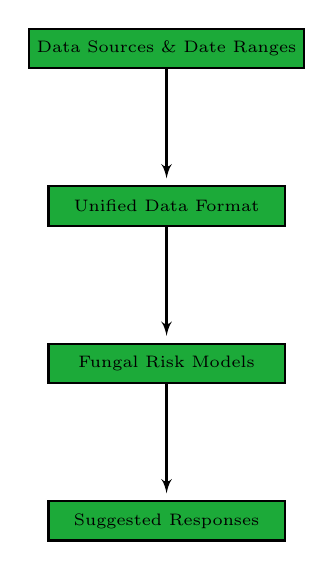
\begin{tikzpicture}[scale=2,node distance=2.5cm,auto,>=latex']
  \mnode{(0,1)}{1.75}{\bh}{Data Sources \& Date Ranges}{a}
  \mnode[(0,-1)]{(a)}{\bw}{\bh}{Unified Data Format}{b}
  \mnode[(0,-1)]{(b)}{\bw}{\bh}{Fungal Risk Models}{c}
  \mnode[(0,-1)]{(c)}{\bw}{\bh}{Suggested Responses}{d}

  \medge{(a)}{(b)}{(0,-\bh/2)}{(0,\bh/2)}
  \medge{(b)}{(c)}{(0,-\bh/2)}{(0,\bh/2)}
  \medge{(c)}{(d)}{(0,-\bh/2)}{(0,\bh/2)}

  \iffalse
  \begin{scope}[on background layer]
    \draw[help lines] (-1.5,-1.5) grid (2,1);
  \end{scope}
  \fi
\end{tikzpicture}
\end{figure}

\clearpage
\pagestyle{empty}

\begin{figure}[!h]
  \centering
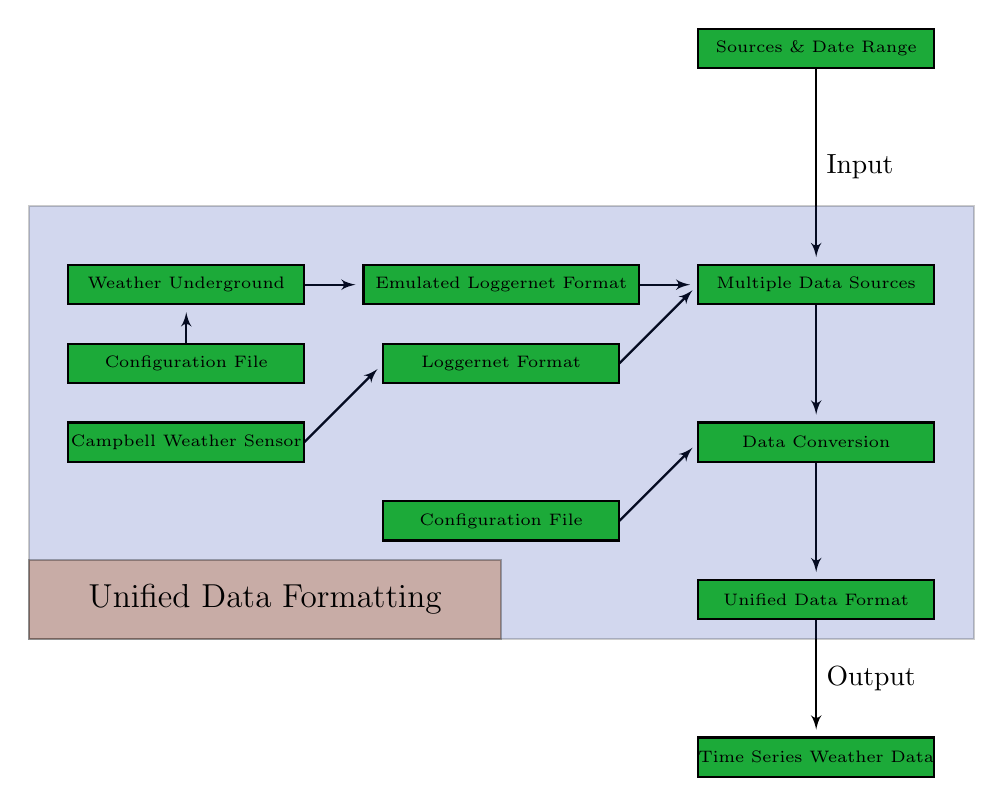
\begin{tikzpicture}[scale=2,node distance=2.5cm,auto,>=latex']
  \draw [fill={rgb:red,5;blue,30;green,10},opacity=0.2,thick] (-3,-1.75) rectangle (3,1);
  \draw [fill={rgb:red,25;blue,0;green,10},opacity=0.3,thick] (-3,-1.75) rectangle (0,-1.25);
  \mtext{(-1.5,-1.5)}{12}{Unified Data Formatting}{n}

  \mnode{(2,-1.5)}{\bw}{\bh}{Unified Data Format}{a}
  \mnode[(0,1)]{(a)}{\bw}{\bh}{Data Conversion}{b}
  \mnode[(-2,-0.5)]{(b)}{\bw}{\bh}{Configuration File}{c}
  \mnode[(0,1)]{(b)}{\bw}{\bh}{Multiple Data Sources}{d}
  \mnode[(-2,0)]{(d)}{1.75}{\bh}{Emulated Loggernet Format}{e}
  \mnode[(-2,-0.5)]{(d)}{\bw}{\bh}{Loggernet Format}{f}
  \mnode[(0,-1)]{(a)}{\bw}{\bh}{Time Series Weather Data}{g}
  \mnode[(0,1.5)]{(d)}{\bw}{\bh}{Sources \& Date Range}{h}
  \mnode[(-2,0)]{(e)}{\bw}{\bh}{Weather Underground}{i}
  \mnode[(-2,-0.5)]{(f)}{\bw}{\bh}{Campbell Weather Sensor}{j}
  \mnode[(0,-0.5)]{(i)}{\bw}{\bh}{Configuration File}{k}

  \medge[Input]{(h)}{(d)}{(0,-\bh/2)}{(0,\bh/2)}
  \medge[Output]{(a)}{(g)}{(0,-\bh/2)}{(0,\bh/2)}
  \medge{(d)}{(b)}{(0,-\bh/2)}{(0,\bh/2)}
  \medge{(b)}{(a)}{(0,-\bh/2)}{(0,\bh/2)}
  \medge{(e)}{(d)}{(\bw/2,0)}{(-\bw/2,0)}
  \medge{(f)}{(d)}{(\bw/2,0)}{(-\bw/2,0)}
  \medge{(c)}{(b)}{(\bw/2,0)}{(-\bw/2,0)}
  \medge{(i)}{(e)}{(\bw/2,0)}{(-0.875,0)}
  \medge{(j)}{(f)}{(\bw/2,0)}{(-\bw/2,0)}
  \medge{(k)}{(i)}{(0,\bh/2)}{(0,-\bh/2)}

  \iffalse
  \begin{scope}[on background layer]
    \draw[help lines] (-3,-3) grid (3,3);
  \end{scope}
  \fi
\end{tikzpicture}
\end{figure}

\clearpage
\pagestyle{empty}

\begin{figure}[!h]
  \centering
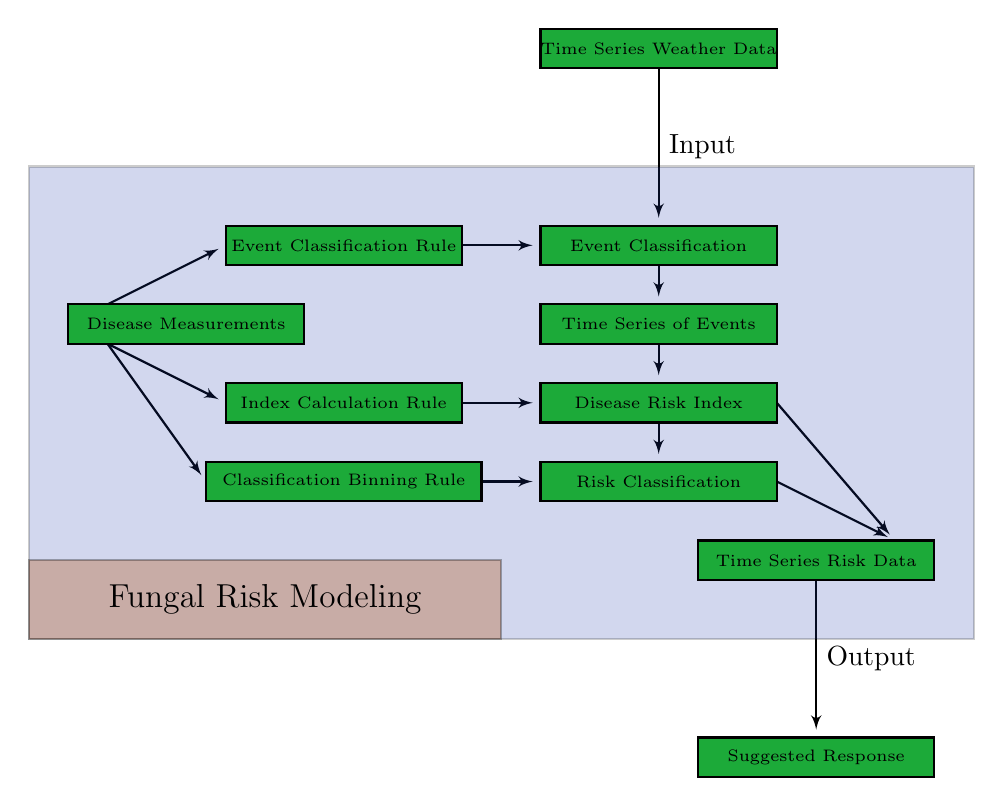
\begin{tikzpicture}[scale=2,node distance=2.5cm,auto,>=latex']
  \draw [fill={rgb:red,5;blue,30;green,10},opacity=0.2,thick] (-3,-1) rectangle (3,2);
  \draw [fill={rgb:red,25;blue,0;green,10},opacity=0.3,thick] (-3,-1) rectangle (0,-0.5);
  \mtext{(-1.5,-0.75)}{12}{Fungal Risk Modeling}{n}

  \mnode{(1,2.75)}{\bw}{\bh}{Time Series Weather Data}{a}
  \mnode[(0,-1.25)]{(a)}{\bw}{\bh}{Event Classification}{b}
  \mnode[(-2,0)]{(b)}{\bw}{\bh}{Event Classification Rule}{c}
  \mnode[(0,-0.5)]{(b)}{\bw}{\bh}{Time Series of Events}{d}
  \mnode[(0,-0.5)]{(d)}{\bw}{\bh}{Disease Risk Index}{e}
  \mnode[(-2,0)]{(e)}{\bw}{\bh}{Index Calculation Rule}{f}
  \mnode[(0,-0.5)]{(e)}{\bw}{\bh}{Risk Classification}{g}
  \mnode[(-2,0)]{(g)}{1.75}{\bh}{Classification Binning Rule}{h}
  \mnode[(-1,0.5)]{(f)}{\bw}{\bh}{Disease Measurements}{k}
  \mnode[(1,-0.5)]{(g)}{\bw}{\bh}{Time Series Risk Data}{i}
  \mnode[(0,-1.25)]{(i)}{\bw}{\bh}{Suggested Response}{j}

  \medge[Input]{(a)}{(b)}{(0,-\bh/2)}{(0,\bh/2)}
  \medge{(b)}{(d)}{(0,-\bh/2)}{(0,\bh/2)}
  \medge{(c)}{(b)}{(\bw/2,0)}{(-\bw/2,0)}
  \medge{(d)}{(e)}{(0,-\bh/2)}{(0,\bh/2)}
  \medge{(f)}{(e)}{(\bw/2,0)}{(-\bw/2,0)}
  \medge{(e)}{(g)}{(0,-\bh/2)}{(0,\bh/2)}
  \medge{(h)}{(g)}{(\bw/2,0)}{(-\bw/2,0)}
  \medge{(e)}{(i)}{(\bw/2,0)}{(0.5,\bh/2)}
  \medge{(g)}{(i)}{(\bw/2,0)}{(0.5,\bh/2)}
  \medge[Output]{(i)}{(j)}{(0,-\bh/2)}{(0,\bh/2)}
  \medge{(k)}{(f)}{(-0.5,-\bh/2)}{(-\bw/2,0)}
  \medge{(k)}{(h)}{(-0.5,-\bh/2)}{(-0.875,0)}
  \medge{(k)}{(c)}{(-0.5,\bh/2)}{(-\bw/2,0)}

  \iffalse
  \begin{scope}[on background layer]
    \draw[help lines] (-3,-2) grid (3,3);
  \end{scope}
  \fi
\end{tikzpicture}
\end{figure}

\end{document}



